\chapter{Introducción}

Un multirrotor es un vehículo aeŕeo no tripulado o UAV (por sus siglas en inglés \textit{Unmanned Aerial Vehicles}) cuyos motores y hélices están orientadas de forma vertical. Estas aeronaves son mucho más maniobrables que una aeronave de ala fija, ya que, al poder mantenerse estables en una posición fija, pueden realizar trayectorias de forma más precisa en espacios reducidos. Comparado con un helicóptero, el cual también puede mantenerse estable en un punto fijo, los multirrotores cuentan con un mantenimiento mucho más sencillo debido a la ausencia de complejos mecanismos.

Generalmente los motores de estas aeronaves son eléctricos, ya que poseen una gran velocidad de reacción y son capaces de manejar una gran cantidad de energía con rendimientos muy elevados. La energía que requieren se proporciona a través de baterías, lo cual limita el tiempo de vuelo de estas aeronaves, cuya autonomía es significativamente inferior a la de las aeronaves de ala fija o a la de los helicópteros con motores de combustión.

Todo esto, unido a su reducido precio, ha permitido que se potencie el uso masivo de este tipo de aeronaves para labores de: agricultura de precisión, topografía, inspección industrial y rodajes cinematográficos, entre otros usos. Existen diversas topologías asociados a los multirrotores, dependiendo del número de motores y la disposición de éstos. En este trabajo se ha desarrollado un cuadricóptero o cuadrirrotor (cuenta con cuatro motores) con disposición en X (\cref{Drone_en_X}).

\begin{figure}[htb!]
		\centering
		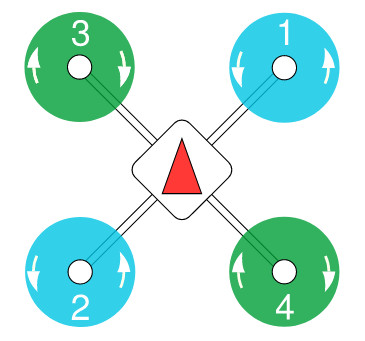
\includegraphics[width=0.3\textwidth]{introduccion/cuadrirrotorX.jpeg}
		\caption{Esquema cuadrirrotor en X}
		\label{Drone_en_X}
	\end{figure}

Se ha escogido un multirrotor de cuatro motores debido a que posee el mínimo numero de motores que permiten un modelo sencillo de la dinámica de la aeronave.

\section{Motivación}

La popularidad de estas aeronaves en ámbitos como la inspección, la topografía o el ámbito cinematográfico requieren que la nave sea muy estable y que se pueda manejar con precisión. Para este propósito, todas estas aeronaves cuentan con un sistema electrónico que se encarga de que la nave sea estable y que facilite el pilotaje de la misma. A este sistema se le conoce como la controladora de vuelo o autopiloto.

\begin{figure}[htb!]
	\centering
	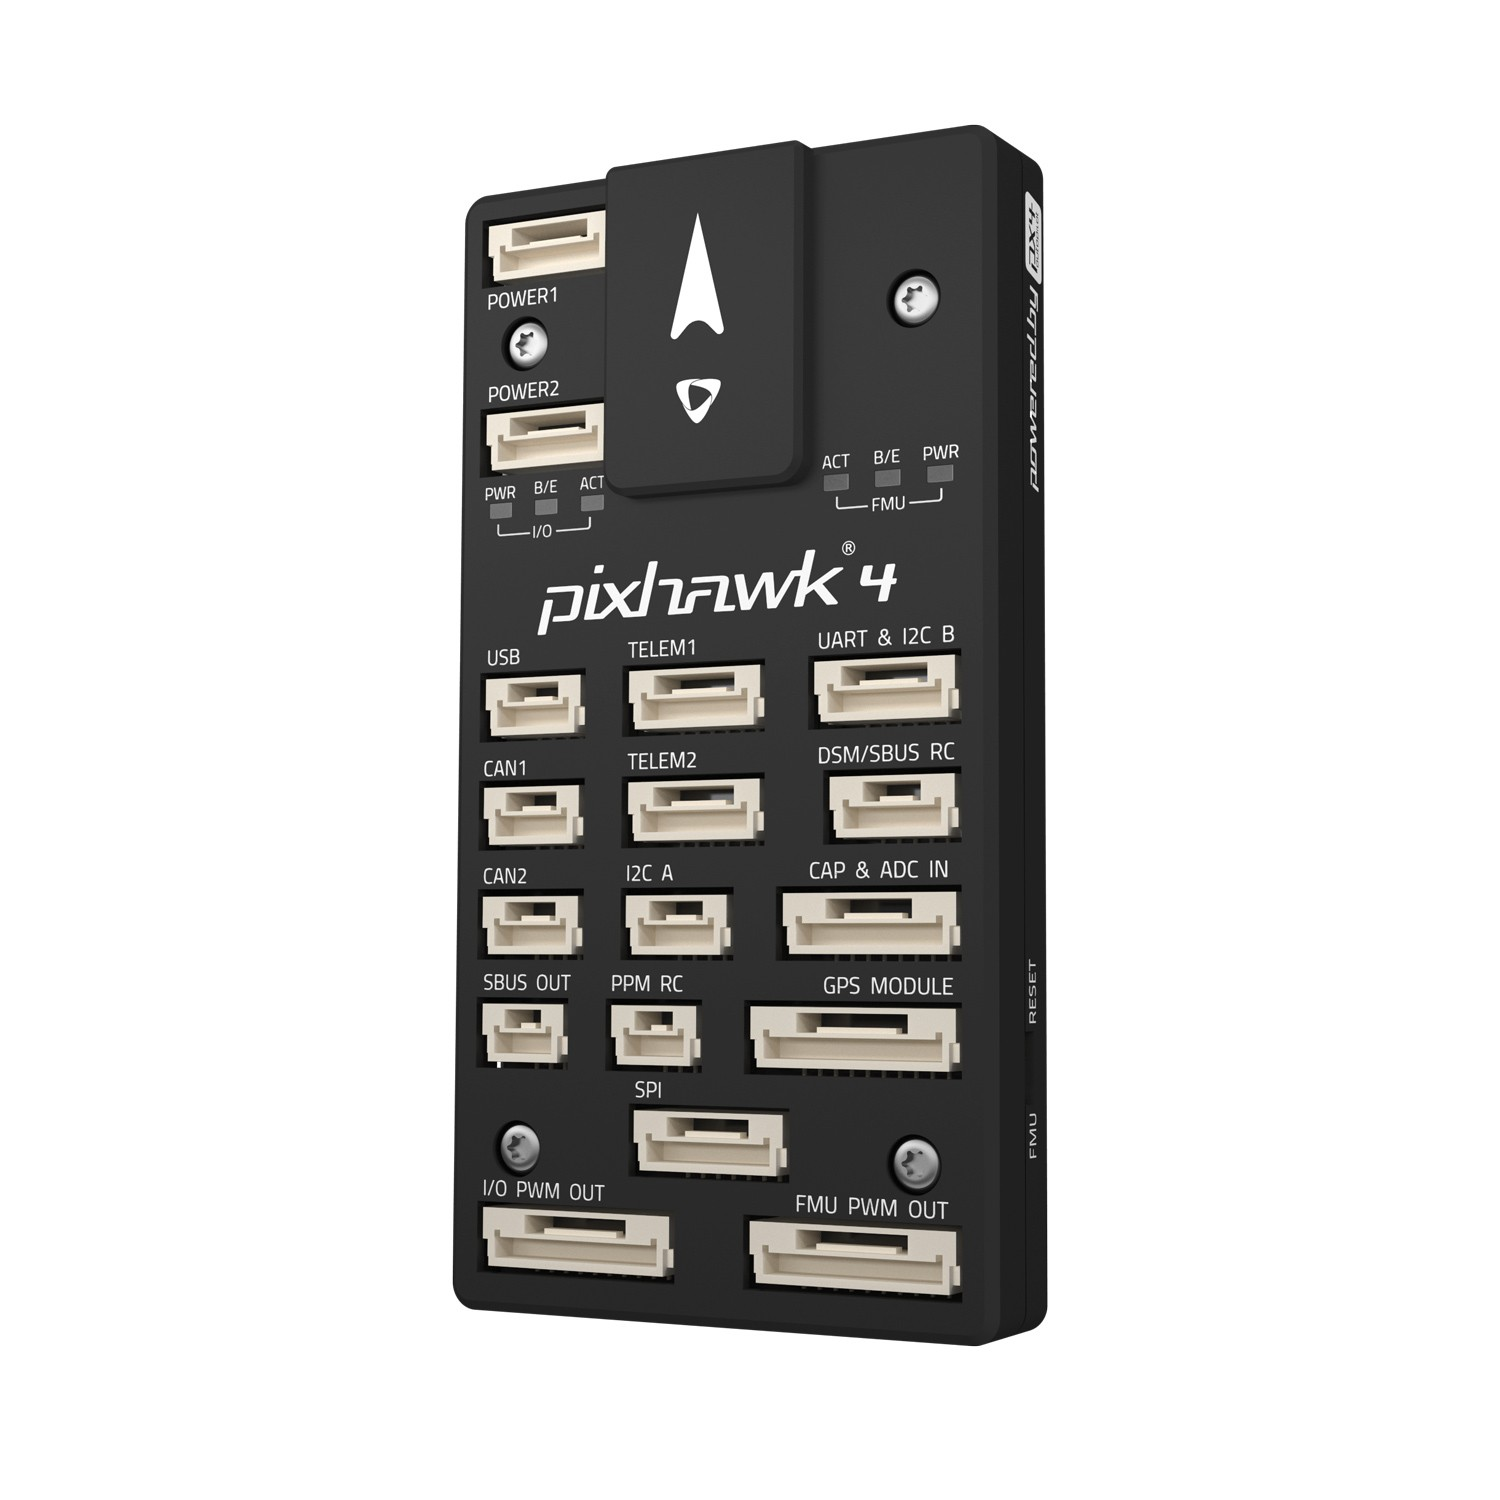
\includegraphics[width=0.3\textwidth]{introduccion/pixhawk4.jpg}
	\caption{Autopiloto comercial Pixhawk 4}
	\label{pixhawk}
\end{figure}

Actualmente, los autopilotos emplean algoritmos de control clásicos, basados la gran mayoría en reguladores PID (Proporcional Integral y Derivativo) para asegurar la estabilidad de la aeronave y permitir que se pilote de forma precisa. Debido a la peligrosidad de los drones (hélices girando a miles de revoluciones por minuto) es altamente complejo probar algoritmos de control novedosos en un cuadricóptero, sin tenerlo anclado a una estructura base, debido a que se trata de un sistema inestable de forma inherente en bucle abierto.

Las teoría clásica de control empleada para estabilizar un cuadricóptero requiere de un conocimiento preciso del modelo del sistema, junto con fino ajuste de los parámetros del controlador. Los últimos avances en aprendizaje automático han permitido que se desarrollen nuevos algoritmos de control empleando técnicas de aprendizaje por refuerzo y redes neuronales.



\section{Solución propuesta}

Con el objetivo de poder desarrollar nuevos algoritmos para el control de cuadrirrotores se ha desarrollado una plataforma, tanto hardware como software, que permita diseñar y probar estos algoritmos de forma segura. Esta plataforma esta constituida de:

\begin{itemize}
	\item \textbf{Entorno de simulación}, sobre el que se puedan probar los algoritmos de control en una aeronave simulada.
	\item \textbf{Cuadrirrotor con autopiloto de diseño propio}, será la aeronave donde se probarán los algoritmos diseñados. Al contar con una controladora de vuelo de diseño propio se pueden implementar los distintos algoritmos de control a bordo.
	\item \textbf{Interfaz con el autopiloto}, el cual comunica a la aeronave con un ordenador, el cual puede enviar comandos a la aeronave y recibir el estado de la misma. Esto permite la implementación de algoritmos \textit{en tierra}, en los cuales la computación del algoritmo se realiza en un ordendador en vez de en el microcontrolador del autopiloto. 
	\item \textbf{Banco de pruebas}, con distintas configuraciones en función del experimento que se desee realizar. Este banco permitirá probar los algoritmos de control de forma segura.
	
\end{itemize}


 Para la validación de la solución propuesta, se ha probado el rendimiento de distintos algoritmos de control basados en técnicas de aprendizaje por refuerzo para poder compararlos con los algoritmos de control clásicos PID.
 
 \section{Objetivos}
 Para poder llevar a cabo esta plataforma y poder implementar algún algoritmo basado en aprendizaje por refuerzo es necesario desgranar los objetivos principales en tareas de alcance más reducido:
 
 \begin{itemize}
 	\item \textbf{Entorno de simulación:}
 	\begin{itemize}
 		\item Estudio del estado del arte acerca de entornos de simulación para el diseño de algoritmos de control para cuadricópteros.
 		\item Estudio del estado del arte acerca de las técnicas de aprendizaje por refuerzo y el control de drones.
 		\item Adaptación del entorno de simulación a la plataforma escogida e integración con ROS.
 		\item Implementación de algoritmos clásicos en el entorno de simulación.
 		\item Diseño de nuevos algoritmos de control basados en aprendizaje por refuerzo y entrenamiento de los mismos.
 		\item Comparativa de los algoritmos en simulación.
 	\end{itemize}
 	\item \textbf{Cuadrirrotor con autopiloto:}
 	\begin{itemize}
 		\item Estudio del estado del arte acerca de los autopilotos comerciales.
 		\item Diseño y construcción completa del autopiloto: componentes, placa de circuito impreso y soldadura de componentes.
 		\item Programación del \textit{firmware} del autopiloto.
 		\item Diseño CAD de los componentes mecánicos del cuadrirrotor e impresion 3D de los mismos.
 		\item Montaje y esamblaje de todos los componentes de la aeronave.  
 	\end{itemize}
 	\item \textbf{Interfaz con el autopiloto:}
 	\begin{itemize}
		\item Diseño del protocolo de comunicación WiFi
		\item Integración del protocolo con ROS y con el autopiloto.
	\end{itemize}
	\item \textbf{Banco de pruebas}:
		\begin{itemize}
			\item Diseño CAD de las piezas de los distintos bancos de pruebas e impresión 3D de las mismas. 
		\end{itemize}
	\item \textbf{Experimentación de los algoritmos en el mundo real:} \tb{reducir o ampliar con los experimentos disponibles}
		\begin{itemize}
			\item Implementación a bordo de los algoritmos cĺásicos.
			\item Implementación externa de los algoritmos clásicos.
			\item Implementacion externa de los algoritmos basados en técnicas de aprendizaje por refuerzo. 
		\end{itemize}
 \end{itemize}
%\newpage
%\section{Estructura de la memoria}